\documentclass[onecolumn,abstract,letter]{scrartcl}
\usepackage[utf8]{inputenc}

% \usepackage[cmintegrals,cmbraces]{newtxmath}
% \usepackage{ebgaramond-maths}

\usepackage{tgpagella}

\usepackage[onehalfspacing]{setspace}
\usepackage[T1]{fontenc}

% \usepackage{baskervillef}
% \usepackage[varqu,varl,var0]{inconsolata}
% \usepackage[scale=.95,type1]{cabin}
% \usepackage[black,t1]{sourceserifpro}
% \usepackage[baskerville,vvarbb]{newtxmath}
% \usepackage[cal=boondoxo]{mathalfa}

\usepackage{mathtools}

\addtokomafont{disposition}{\rmfamily}
\addtokomafont{section}{\textsc}

% \RedeclareSectionCommand[style=section,indent=0pt]{part}
% \renewcommand*{\partformat}{\thepart\enskip}

\renewcommand{\thesection}{\Roman{section}} 
\renewcommand{\thesubsection}{\Alph{subsection}}
\renewcommand{\thesubsubsection}{\arabic{subsection}}



\title{\textsc{\textmd{Statistical Learning Methodology in Material Science}}}
\author{Draft - Julien Brenneck}
\date{June 2018}

\begin{document}

\maketitle

%%%%%%%%%%%%%%%%%%%%%%%%%%%%%%%%%%%%%%%%%%%%%%%%%%
%%%%%%%%%%%%%%%%%%%%%%%%%%%%%%%%%%%%%%%%%%%%%%%%%%

% \begin{abstract}

% Material Science faces the insurmountable cost of experimentally collecting the properties of endless potential materials. 
% Computational techniques based on \textit{ab initio} simulation alleviate this burden, increasing the number of categorized materials by (?) orders of magnitude. 
% The computational cost of these techniques makes it still unfeasible to test all potential materials even in limited domains. 
% Models from statistics and machine learning are poised to utilize existing datasets to advance the search for new materials, as well as further the understanding of existing data.
% This paper attempts to highlight pitfalls and best practices in the use of these models. 


% \end{abstract}

%%%%%%%%%%%%%%%%%%%%%%%%%%%%%%%%%%%%%%%%%%%%%%%%%%
%%%%%%%%%%%%%%%%%%%%%%%%%%%%%%%%%%%%%%%%%%%%%%%%%%

\begin{section}{Introduction}
Material Science faces the problem of experimentally collecting the properties of endless materials. 
Computational techniques based on \textit{ab initio} simulation alleviate this burden, increasing the ability to categorize materials by (?) orders of magnitude. 
The computational cost of these techniques makes it still unfeasible to test all potential materials even in limited domains, necessitating efficient higher level models of materials and their properties. 
Models from statistics and machine learning promise to utilize existing datasets to advance the search for new materials, as well as further the understanding of existing data.
This paper attempts to highlight pitfalls and best practices in the use of these models. 

The fundamental issue in choosing statistical and machine learning models is ensuring that the model learns to generalize.
A sufficiently powerful model may simply memorize local noise inherent to the training set without learning the overall trends in data, and hence would perform poorly on new data. 
While material science has begun to adopt these models, there has been less adoption of rigorous validation methodology.
This work examines the main methods of statistical and machine learning, such as the hold out test set, cross-validation, and the bootstrap. 
While simple to implement, care must be taken in the application of these methods to avoid inadvertent and potentially invalidating bias in the results. 
Use of best practices, publishing of models and hyper-parameters and reproducible in general, builds the confidence of a result. 

\end{section}

%%%%%%%%%%%%%%%%%%%%%%%%%%%%%%%%%%%%%%%%%%%%%%%%%%
%%%%%%%%%%%%%%%%%%%%%%%%%%%%%%%%%%%%%%%%%%%%%%%%%%

\begin{section}{Materials \& Methods}

The experiments in this study were run using scikit-Learn (0.19.1) with Python (3.6.5) on NERSC jupyterhub computing resources. All jupyter notebooks to be available in supplementary materials. 
Additional data comes from Matminer (0.3.5).

\begin{subsection}{Cross-Validation}

\begin{subsubsection}{Experiment 1}
Highlighting the bias variance trade-off in the choice of $K$ for $K$-fold cross validation (CV) is difficult due to the fundamental inability to fully quantify CV variance, as there is no unbiased statistical estimator and the bias can in practice be on the order of magnitude as the variance itself.
Despite this, it is possible to show the overall trends inherent to the choice of $K$, as the bias will decrease and variance will increase significantly as $K$ increases, even if the exact values are poor estimators of the true variance. 
Understanding the variance of CV is critical to understanding how the model will generalize, the ultimate goal of training such a model.
If the true model variance is high, we would expect there to be large changes in the model for small perturbations in the data, meaning the model has fit itself to noise.

This experiment computes the $K$-fold CV scores of a Support Vector Machine (SVM) using Radial Basis Function (RBF) kernel regression, for all possible values of $K$, that is $2$ to $N$ where $N$ is the number of samples.
The special case of $N=K$ is also called Leave One Out Cross Validation (LOOCV).
The CV error is estimated as the sample mean of all $K$ folds.
% \begin{equation}
%     Err_{CV} = \frac{1}{N}\sum_{i=1}^{K} L()
% \end{equation}
The $D$ dimensional input data is generated from independent Normal distributions in each dimension.
The $1$ dimensional output data for regression is the product of the sine of each dimension, with gaussian noise added.
\begin{equation}
    Y_i = \prod_{j=1}^{D} \sin(X_{i,j}) + \epsilon
\end{equation}
The variance can be estimated as the sample variance of the folds. See figure \ref{fig:kfold-cv}.
\end{subsubsection}

\begin{figure}[h]
    \centering
    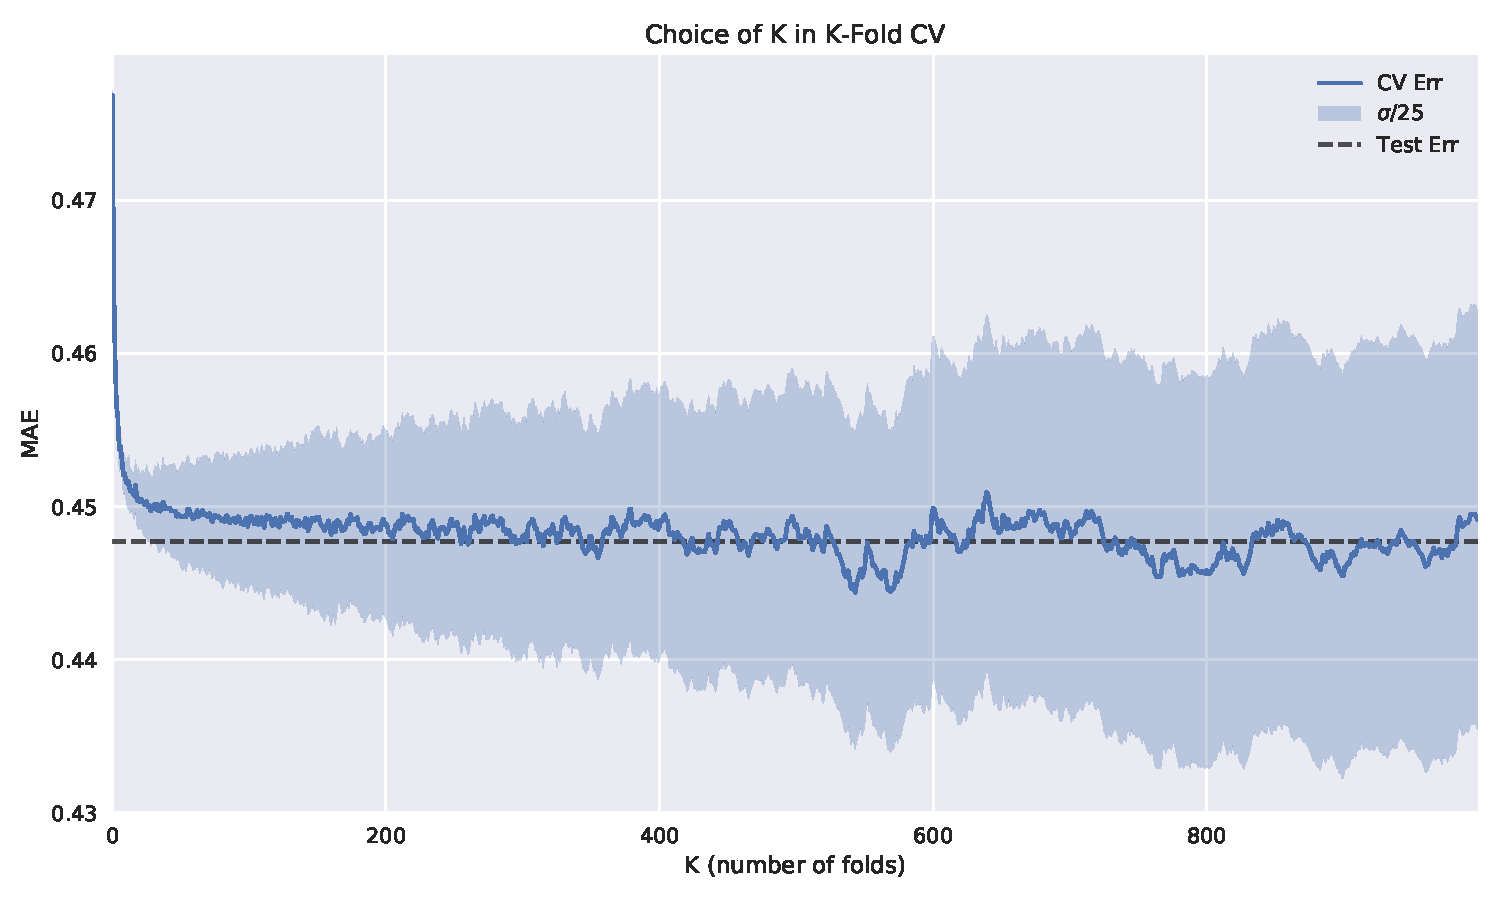
\includegraphics[width=\linewidth]{kfold-cv-std-10x6.eps}
    \caption{Effects of varying $K$ in $K$-Fold cross-validation. (These shouldn't all be the same blue, will fix this)}
    \label{fig:kfold-cv}
\end{figure}

\begin{subsubsection}{Experiment 2}
A more straightforward way of measuring variance relies on knowing the underlying distribution, or at the least having incredibly large amounts of data compared to its complexity. 
Instead of taking variance of the scores from each fold, the model can be trained on new data from the same underlying distribution multiple times, and the sample variance of CV estimates can be taken.
This more intuitively estimates the true model variance, but is computationally more expensive by at least one order of magnitude. 
This can be accomplished simply by repeating Experiment 1 multiple times with new data sets. 

\end{subsubsection}

\begin{subsubsection}{Experiment 3}
In the context of model selection, model variance can be measured through the variance of the model selected.
In practice this means using CV to select a continuous hyper-parameter, and taking the sample variance of selected hyper-parameters.

The same data and model is used as in the previous experiments.
The selected hyper-parameter is $\gamma$.
Raising the value of $\gamma$ effectively increases the complexity of the model, allowing it to capture more details of the data.
A grid search on $(10^{-4}, 10^{4})$ is used with $K$-fold cross validation, with value of $K$ of $2,5,10,$ and $N$.
For each value of $K$ a grid search is performed on a new data set sampled from the underlying distribution several times, and the sample variance of $\gamma$ values selected is taken.

\end{subsubsection}

\end{subsection}


\end{section}



%%%%%%%%%%%%%%%%%%%%%%%%%%%%%%%%%%%%%%%%%%%%%%%%%%
%%%%%%%%%%%%%%%%%%%%%%%%%%%%%%%%%%%%%%%%%%%%%%%%%%

% \begin{section}{Model Selection and Evaluation}

% \end{section}

%%%%%%%%%%%%%%%%%%%%%%%%%%%%%%%%%%%%%%%%%%%%%%%%%%
%%%%%%%%%%%%%%%%%%%%%%%%%%%%%%%%%%%%%%%%%%%%%%%%%%

% \begin{section}{Cross Validation}

% \end{section}

%%%%%%%%%%%%%%%%%%%%%%%%%%%%%%%%%%%%%%%%%%%%%%%%%%
%%%%%%%%%%%%%%%%%%%%%%%%%%%%%%%%%%%%%%%%%%%%%%%%%%

\scriptsize
\nocite{*}
\bibliography{MLMS}
\bibliographystyle{plain}

\end{document}
